
\chapter{无线信号调制识别以及深度学习理论}
\label{chap: mod_rec_deep_learning_theo}
\section{引言}

\section{调制识别}
\subsection{调制信号}
\label{sec:mod_signal}
在动态频谱接入中,执行的关键传感之一是提供对附近发射器的了解,以避免无线电干扰并优化频谱分配。这种识别和区分广播无线电,本地和广域数据和语音无线电,雷达用户以及其他附近潜在的无线电干扰源都有不同的行为和要求。然后,调制识别将接收到的无线电信号的调制类型分类为了解何种类型的通信方案和发射器存在的步骤。\par

本文针对的调制信号有。。。

\subsection{调制信息}
在无线电通信中,信号通常由定义好的和理解的基本功能上的许多调制数据位组成由这些基地形成的离散模式。信号的复合基带表示将无线电电压电平时间序列分解为其对载波频率的正弦和余弦函数的投影。通过操纵频率,幅度,相位或其总和,数据比特然后通过离散和可分离的模式调制到这个空间中,对于数字的每个不同的符号周期,或者在模拟调制的情况下连续的位置。对于QPSK的情况,这个相位映射如4所示。然后通常将脉冲整形滤波器(例如根升余弦)应用于频带限制信号,并消除这些不同模式之间的尖锐宽带瞬态,导致相邻符号在发射机处的基极以确定性和可逆性混合。在我们的模拟数据集中,我们使用一个根升余弦脉冲整形滤波器,每个数字信号的带宽为0.35。\par

\subsection{信道对调制信号的影响}
在传播效应的这些苛刻的现实假设下,对专家特征和决策度量的最优性进行分析建模是非平凡的,并且经常会使得简化假设。 在本文中,我们将重点放在包括所有上述效应在内的苛刻的模拟传播环境中的性能的经验性测量,但不要尝试以封闭形式分析追踪其性能。\par

相比之下,信道效应不是确定性的,在通信系统中不是完全可逆的。真实的系统在传输的信号上经历许多影响,这使得恢复和表示具有挑战性。热噪声在接收器处产生相对平坦的高斯白噪声,其形成本底噪声或灵敏度级别和信噪比。由于温度和其他半导体物理因发射器和接收器的不同而引起的振荡器漂移导致符号时序偏移,采样速率偏移,载波频率偏移和相位差。这些效应导致信道之间的时间移位,缩放,线性混合/旋转以及基于未知时变过程的接收信号的旋转。最后,根据在接收机处发射信号的到达模式,实际信道经历随机滤波,具有不同的幅度,相位,多普勒和延迟。这是一种通常被称为多径衰落或频率选择性衰落的现象,其发生在信号可能反射出建筑物,车辆或环境中的任何形式的反射器的任何环境中。通常在接收机中通过估计时变信道响应的瞬时值并将其从接收信号解卷积来消除这种情况。\par

\section{神经网络概述}
\subsection{神经元概述}
以监督学习为例,假设我们有训练样本集$(x(^i),y(^i))$,那么神经网络算法能够提供一种复杂且非线性的假设模型$h_{W,b}(x)$ ,它具有参数$W, b$,可以以此参数来拟合我们的数据。图\ref{fig_2_1}即是“神经元”的图示:\par
\begin{figure}[htbp]
	\centering
	% Requires \usepackage{graphicx}
	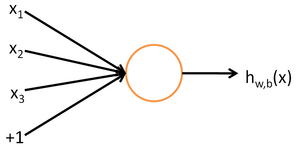
\includegraphics[scale=0.5]{figures/chapter_2/SingleNeuron.png}\\
	\caption{神经元示意图}\label{fig_2_1}
\end{figure}
这个“神经元”是一个以$x_1, x_2, x_3$ 及截距$+1$ 为输入值的运算单元,其输出为:
\begin{equation}
	h_{W,b}(x) = f(W^Tx) = f(\sum_{i=1}^3 W_{i}x_i +b)
\end{equation} 
其中函数$f : \Re \mapsto \Re$被称为“激活函数”。在本教程中,我们选用sigmoid函数作为激活函数$f(\cdot)$
\begin{equation}
	f(z) = \frac{1}{1+\exp(-z)}.
\end{equation}
可以看出,这个单一“神经元”的输入-输出映射关系其实就是一个逻辑回归(logistic regression)。\par
虽然本系列教程采用sigmoid函数,但你也可以选择双曲正切函数(tanh):\par
\begin{equation}
f(z) = \tanh(z) = \frac{e^z - e^{-z}}{e^z + e^{-z}}
\end{equation}
$\tanh(z)$函数是sigmoid函数的一种变体,它的取值范围为$[-1,1]$ ,而不是sigmoid函数的$[0,1]$ 。\par
图\ref{fig_2_2}分别是sigmoid及tanh的函数图像:
\begin{figure}[!h]
	\centering
	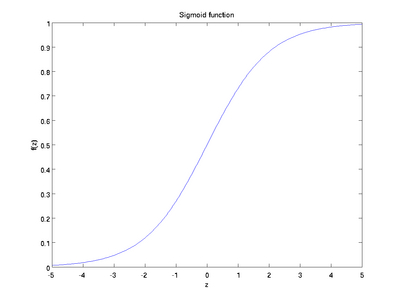
\includegraphics[scale=0.8]{figures/chapter_2/Sigmoid_Function.png}
	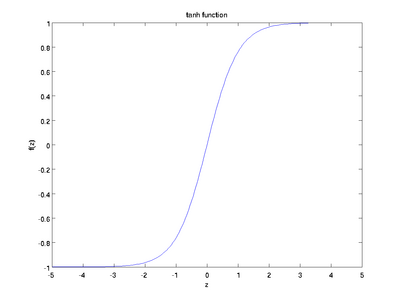
\includegraphics[scale=0.8]{figures/chapter_2/Tanh_Function.png}
	\caption{sigmoid函数与tanh函数}\label{fig_2_2}
\end{figure}

\subsection{前馈神经网络}
前馈神经网络就是将许多个单一“神经元”联结在一起,这样,一个“神经元”的输出就可以是另一个“神经元”的输入。例如,图\ref{fig_2_3}就是一个简单的神经网络:
\begin{figure}
	\centering
	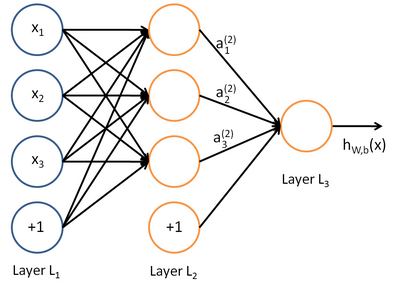
\includegraphics[scale=0.5]{figures/chapter_2/Network.png}
	\caption{前馈神经网络}\label{fig_2_3}
\end{figure}
我们使用圆圈来表示神经网络的输入,标上“$+1$”的圆圈被称为偏置节点,也就是截距项。神经网络最左边的一层叫做输入层,最右的一层叫做输出层(本例中,输出层只有一个节点)。中间所有节点组成的一层叫做隐藏层,因为我们不能在训练样本集中观测到它们的值。同时可以看到,以上神经网络的例子中有3个输入单元(偏置单元不计在内),3个隐藏单元及一个输出单元。\par

 我们用 来表示网络的层数,本例中 ,我们将第 层记为 ,于是 是输入层,输出层是 。] 我们用$a^{(l)}_i$表示第$l$层第$i$单元的激活值(输出值)。当$l=1$时,$a^{(1)}_i = x_i$,也就是第$i$个输入值(输入值的第$i$个特征)。对于给定参数集合$W,b$,我们的神经网络就可以按照函数$h_{W,b}(x)$来计算输出结果。\par
 
我们用$z^{(l)}_i$表示第$l$层第$i$单元输入加权和(包括偏置单元)

我们将上面的计算步骤叫作前向传播。回想一下,之前我们用$a^{(1)} = x$表示输入层的激活值,那么给定第$l$层的激活值$a^{(l)}$后,第$l+1$层的激活值$a^{(l+1)}$就可以按照下面步骤计算得到:
\begin{align}
	z^{(l+1)} &= W^{(l)} a^{(l)} + b^{(l)}=\sum_{j=l}^n W^{(l)}_{ij} x_j + b^{(l)}_i\\
	a^{(l+1)} &= f(z^{(l+1)})
\end{align}
将参数矩阵化,使用矩阵-向量运算方式,我们就可以利用线性代数的优势对神经网络进行快速求解。\par

目前为止,我们讨论了一种神经网络,我们也可以构建另一种结构的神经网络(这里结构指的是神经元之间的联接模式),也就是包含多个隐藏层的神经网络。最常见的一个例子是$n_l$层的神经网络,第$1$ 层是输入层,第$n_l$层是输出层,中间的每个层$l$与层$l+1$紧密相联。这种模式下,要计算神经网络的输出结果,我们可以按照之前描述的等式,按部就班,进行前向传播,逐一计算第$L_2$层的所有激活值,然后是第$L_3$层的激活值,以此类推,直到第$L_{n_l}$ 层。这是一个前馈神经网络的例子,因为这种联接图没有闭环或回路。\par

\subsection{反向传播算法}
假设我们有一个固定样本集$\{ (x^{(1)}, y^{(1)})$, $\ldots$, $(x^{(m)}$, $y^{(m)}) \}$,它包含$m$个样例。我们可以用批量梯度下降法来求解神经网络。具体来讲,对于单个样例$(x,y)$,我们假设其代价函数$J(W,b; x,y)$为方差代价函数,则有:
\begin{align}
	J(W,b; x,y) = \frac{1}{2} \left\| h_{W,b}(x) - y \right\|^2.
\end{align}
给定一个包含$m$个样例的数据集,那么整体代价函数$J(W,b)$为:
\begin{equation}
	\begin{aligned}
	J(W,b)
	&= \left[ \frac{1}{m} \sum_{i=1}^m J(W,b;x^{(i)},y^{(i)}) \right]
	+ \frac{\lambda}{2} \sum_{l=1}^{n_l-1} \; \sum_{i=1}^{s_l} \; \sum_{j=1}^{s_{l+1}} \left( W^{(l)}_{ji} \right)^2
	\\
	&= \left[ \frac{1}{m} \sum_{i=1}^m \left( \frac{1}{2} \left\| h_{W,b}(x^{(i)}) - y^{(i)} \right\|^2 \right) \right]
	+ \frac{\lambda}{2} \sum_{l=1}^{n_l-1} \; \sum_{i=1}^{s_l} \; \sum_{j=1}^{s_{l+1}} \left( W^{(l)}_{ji} \right)^2
	\end{aligned}
\end{equation}
以上关于$J(W,b)$定义中的第一项是一个均方差项。第二项是一个规则化项(也叫权重衰减项),其目的是减小权重的幅度,防止过度拟合。
权重衰减参数$\lambda$用于控制公式中两项的相对重要性。

以上的代价函数经常被用于分类和回归问题。在分类问题中,我们用$y=0$或$1$,来代表两种类型的标签(回想一下,这是因为sigmoid激活函数的值域为$[0,1]$;如果我们使用双曲正切型激活函数,那么应该选用$-1$和$+1$ 作为标签)。对于回归问题,我们首先要变换输出值域,以保证其范围为$[0,1]$(同样地,如果我们使用双曲正切型激活函数,要使输出值域为$[-1,1]$)。\par

反向传播算法的思路如下:给定一个样例$(x,y)$,我们首先进行“前向传导”运算,计算出网络中所有的激活值,包括$h_{W,b}(x)$的输出值。之后,针对第$l$层的每一个节点$i$,我们计算出其“残差”$\delta^{(l)}_i$,该残差表明了该节点对最终输出值的残差产生了多少影响。对于最终的输出节点,我们可以直接算出网络产生的激活值与实际值之间的差距,我们将这个差距定义为$\delta^{(n_l)}_i$(第$n_l$层表示输出层)。对于隐藏单元我们如何处理呢?我们将基于节点残差的加权平均值计算$\delta^{(l)}_i$,这些节点以$a^{(l)}_i$作为输入。反向传播算法可表示为以下几个步骤:\par
进行前馈传导计算,利用前向传导公式,得到$L_2, L_3$, $\ldots$直到输出层$L_{n_l}$的激活值。
对输出层(第$n_l$层),计算:
\begin{align}
	\delta^{(n_l)}
	= - (y - a^{(n_l)}) \bullet f'(z^{(n_l)})
\end{align}
对于$l = n_l-1, n_l-2, n_l-3$, $\ldots$, $2$的各层,计算:
\begin{align}
	\delta^{(l)} = \left((W^{(l)})^T \delta^{(l+1)}\right) \bullet f'(z^{(l)})
\end{align}
计算最终需要的偏导数值:
\begin{align}
	\nabla_{W^{(l)}} J(W,b;x,y) &= \delta^{(l+1)} (a^{(l)})^T, \\
	\nabla_{b^{(l)}} J(W,b;x,y) &= \delta^{(l+1)}.
\end{align}
实现中应注意:在以上的第2步和第3步中,我们需要为每一个$i$值计算其$f'(z^{(l)}_i)$。假设$f(z)$是sigmoid函数,并且我们已经在前向传导运算中得到了$a^{(l)}_i$。
最后,我们将对梯度下降算法做个全面总结。在下面的伪代码中,$\Delta W^{(l)}$是一个与矩阵$W^{(l)}$维度相同的矩阵,$\Delta b^{(l)}$是一个与$b^{(l)}$维度相同的向量。注意这里“$\Delta W^{(l)}$”是一个矩阵,而不是“$ \Delta$与$W^{(l)}$相乘”。下面,我们实现批量梯度下降法中的一次迭代:\par

对于所有$l$,令$\Delta W^{(l)} := 0$, $\Delta b^{(l)} := 0 $(设置为全零矩阵或全零向量)
对于$i = 1$到$m$,
使用反向传播算法计算$\nabla_{W^{(l)}} J(W,b;x,y)$和$\nabla_{b^{(l)}} J(W,b;x,y)$。
计算$\Delta W^{(l)} := \Delta W^{(l)} + \nabla_{W^{(l)}} J(W,b;x,y)$。
计算$\Delta b^{(l)} := \Delta b^{(l)} + \nabla_{b^{(l)}} J(W,b;x,y)$。
更新权重参数:
\begin{align}
	W^{(l)} &= W^{(l)} - \alpha \left[ \left(\frac{1}{m} \Delta W^{(l)} \right) + \lambda W^{(l)}\right] \\
	b^{(l)} &= b^{(l)} - \alpha \left[\frac{1}{m} \Delta b^{(l)}\right]
\end{align}
现在,我们可以重复梯度下降法的迭代步骤来减小代价函数$J(W,b)$的值,进而求解我们的神经网络。

\section{卷积神经网络}
卷积网络,也叫做卷积神经网络,是一种专门用来处理具有类似网格结构的数据的神经网络。
例如时间序列数据(可以认为是在时间轴上有规律地采样形成的一维网格)和图像数据(可以看作是二维的像素网格)。
卷积网络在诸多应用领域都表现优异。卷积是一种特殊的线性运算。
\emph{卷积网络是指那些至少在网络的一层中使用卷积运算来替代一般的矩阵乘法运算的神经网络。}\par

\subsection{卷积运算}
\label{sec:the_convolution_operation}

卷积是对两个实变函数的一种数学运算,通常我们用星号表示:
\begin{equation}
s(t) = (x*w)(t) = \int x(\tau)w(t-\tau)d\tau
\end{equation}

在卷积网络的术语中,卷积的第一个参数(在这个例子中,函数$x$)通常叫做输入,第二个参数(函数$w$)叫核函数。
输出有时被称作特征映射。

如果我们假设$x$和$w$都定义在整数时刻$t$上,则卷积的离散形式:
\begin{equation}
s(t) = (x*w)(t) = \sum_{\tau = -\infty}^{\infty} x(\tau)w(t\tau).
\end{equation}

在机器学习的应用中,输入通常是多维数组的数据,而核通常是由学习算法优化得到的多维数组的参数。
我们把这些多维数组叫做张量。
因为在输入与核中的每一个元素都必须明确地分开存储,我们通常假设在存储了数值的有限点集以外,这些函数的值都为零。
这意味着在实际操作中,我们可以通过对有限个数组元素的求和来实现无限求和。

在处理图像数据时,我们经常一次在多个维度上进行卷积运算。如果把一张二维的图像$I$作为输入,同时使用使用一个二维的核$K$,则有:
\begin{equation}
S(i,j) = (I*K)(i,j) = \sum_m \sum_n I(m,n) K(i-m, j-n).
\end{equation}

卷积是可交换的(commutative),我们可以等价地写作:
\begin{equation}
S(i, j) = (K*I)(i,j) = \sum_m \sum_n I(i-m, j-n) K(m, n).
\end{equation}

卷积运算可交换性的出现是因为我们将核相对输入进行了翻转,从$m$增大的角度来看,输入的索引在增大,但是核的索引在减小。
我们将核翻转的唯一目的是实现可交换性。
许多神经网络库会实现一个相关的函数,称为互相关函数,和卷积运算几乎一样但是并没有对核进行翻转:
\begin{equation}
S(i, j) = (I*K)(i, j) = \sum_m \sum_n I(i+m, j+n) K(m, n).
\end{equation}
许多机器学习的库实现的是互相关函数但是称之为卷积,在本文中,我们将这两种运算都称之为卷积运算。\par

\subsection{卷积特性}
卷积运算通过三个重要的思想来帮助改进机器学习系统:稀疏交互、参数共享、等变表示。

传统的神经网络使用矩阵乘法来建立输入与输出的连接关系。
对于卷积,参数共享的特殊形式使得神经网络层具有对平移等变的性质。
如果一个函数满足输入改变,输出也以同样的方式改变这一性质,我们就说它是等变(equivariant)的。
特别地,如果函数$f(x)$与$g(x)$满足$f(g(x))= g(f(x))$,我们就说$f(x)$对于变换$g$具有等变性。
对于卷积来说,如果令$g$是输入的任意平移函数,那么卷积函数对于$g$具有等变性。
当处理时间序列数据时,这意味着通过卷积可以得到一个由输入中出现不同特征的时刻所组成的时间轴。
如果我们把输入中的一个事件向后延时,在输出中仍然会有完全相同的表示,只是时间延后了。
而这也正好对应到我们无线信号中的时移不变性。因此,我们可以很好的将\label{con_net}应用到调制信号识别中。\par

\subsection{卷积作为一种无限强的先验}
先验被认为是强或者弱取决于先验中概率密度的集中程度。
弱先验具有较高的熵值,例如方差很大的高斯分布。这样的先验允许数据对于参数的改变具有或多或少的自由性。
强先验具有较低的熵值,例如方差很小的高斯分布。这样的先验在决定参数最终取值时起着更加积极的作用。
一个无限强的先验需要对一些参数的概率置零并且完全禁止对这些参数赋值,无论数据对于这些参数的值给出了多大的支持。\par

我们可以把卷积网络类比成全连接网络,但对于这个全连接网络的权重有一个无限强的先验。
这个无限强的先验是说一个隐藏单元的权重必须和它邻居的权重相同,但可以在空间上移动。
这个先验也要求除了那些处在隐藏单元的小的空间连续的接受域内的权重以外,其余的权重都为零。

总之,我们可以把卷积的使用当作是对网络中一层的参数引入了一个无限强的先验概率分布。
这个先验说明了该层应该学得的函数只包含局部连接关系并且对平移具有等变性。

\subsection{随机或无监督的特征}
\label{sec:random_or_unsupervised_features}

通常,卷积网络训练中最耗时的部分是学习特征。 
输出层的计算代价通常相对不高,因为在通过若干层卷积池化之后作为该层输入的特征的数量较少。
当使用梯度下降执行监督训练时,每步梯度计算需要完整地运行整个网络的前向传播和反向传播。
减少卷积网络训练成本的一种方式是使用那些不是由监督方式训练得到的特征。\par

有三种基本策略可以不通过监督训练而得到卷积核。
其中一种是简单地随机初始化它们。
另一种是手动设计它们,例如设置每个核在一个特定的方向或尺度来检测边缘。
最后,可以使用无监督的标准来学习核。\par

使用无监督的标准来学习特征,允许这些特征的确定与位于网络结构顶层的分类层相分离。
然后只需提取一次全部训练集的特征,构造用于最后一层的新训练集。
假设最后一层类似逻辑回归或者支持向量机,那么学习最后一层通常是凸优化问题。\par


随机过滤器经常在卷积网络中表现得出乎意料得好~\cite{Jarrett-ICCV2009-small,Saxe-ICML2011,pinto2011scaling,cox2011beyond}。
\cite{Saxe-ICML2011}~说明,由卷积和随后的池化组成的层,当赋予随机权重时,自然地变得具有频率选择性和平移不变性。
他们认为这提供了一种廉价的方法来选择卷积网络的结构:首先通过仅训练最后一层来评估几个卷积网络结构的性能,然后选择最好的结构并使用更昂贵的方法来训练整个网络。
一个中间方法是学习特征,但是使用那种不需要在每个梯度计算步骤中都进行
完整的前向和反向传播的方法。与多层感知机一样,我们使用贪心逐层预训练,单
独训练第一层,然后一次性地从第一层提取所有特征,之后用那些特征单独训练
第二层,以此类推。



\section{卷积降噪自编码器}
自编码器可以理解为一个试图去还原其原始输入的系统。如下图所示。
\begin{figure}[!h]
	\centering
	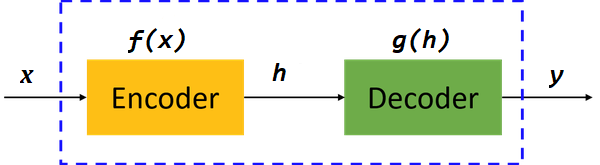
\includegraphics[scale=0.8]{figures/chapter_3/AE}
	\caption{自编码器}	\label{fig_3_2}
\end{figure}

图中,虚线蓝色框内就是一个自编码器模型,它由编码器(Encoder)和解码器(Decoder)两部分组成,本质上都是对输入信号做某种变换。编码器将输入信号x变换成编码信号y,而解码器将编码信号y转换成输出信号。即:
\begin{equation}
	\begin{gathered}
		y=f(x)
		\\
		x=g(y)=g(f(x))
	\end{gathered}
\end{equation}
而自编码器的目的是,让输出尽可能复现输入x。对于自编码器,我们往往并不关心输出是什么(反正只是复现输入),我们真正关心的是中间层的编码信号,或者说是从输入到编码的映射。在我们强迫编码信号y和输入信号x不同的情况下,系统还能够去复原原始信号x,那么说明编码信号y已经承载了原始数据的所有信息,但以一种不同的形式,这便是特征提取。对于卷积自便器,我们中间的隐层是利用卷积网络实现的。\par

在自编码器的训练过程中,我们尽量减少重构均方误差(MSE),但由于我们的主要目标是获得一个良好的聚类稀疏表示,我们显着限制隐藏层维度到一个点,我们的重构作出一些可见的简化假设,在最优重构误差下降低了隐层维数。图3显示了两个训练样例,2x128输入向量的样子,1x30稀疏表示的样子,以及2x128输出重构的样子。这给了这个网络的学习代表能力的一些直觉。\par


\section{\glssymbol{LSTM}}
\label{sec:lstm}
\label{chap:sequence_modeling_recurrent_and_recursive_nets}
\gls{RNN}或~\glssymbol{RNN}是一类用于处理序列数据的\gls{NN}。
就像\gls{convolutional_network}是专门用于处理网格化数据的\gls{NN},\gls{RNN}是专门用于处理序列$x^{(1)}, \dots, x^{(\tau)}$的\gls{NN}。

正如\gls{convolutional_network}可以很容易地扩展到具有很大宽度和高度的图像,以及处理大小可变的图像,\gls{recurrent_network}可以扩展到更长的序列(比不基于序列的特化网络长得多)。
大多数\gls{recurrent_network}也能处理可变长度的序列。

\begin{figure}[!h]
	\centering
	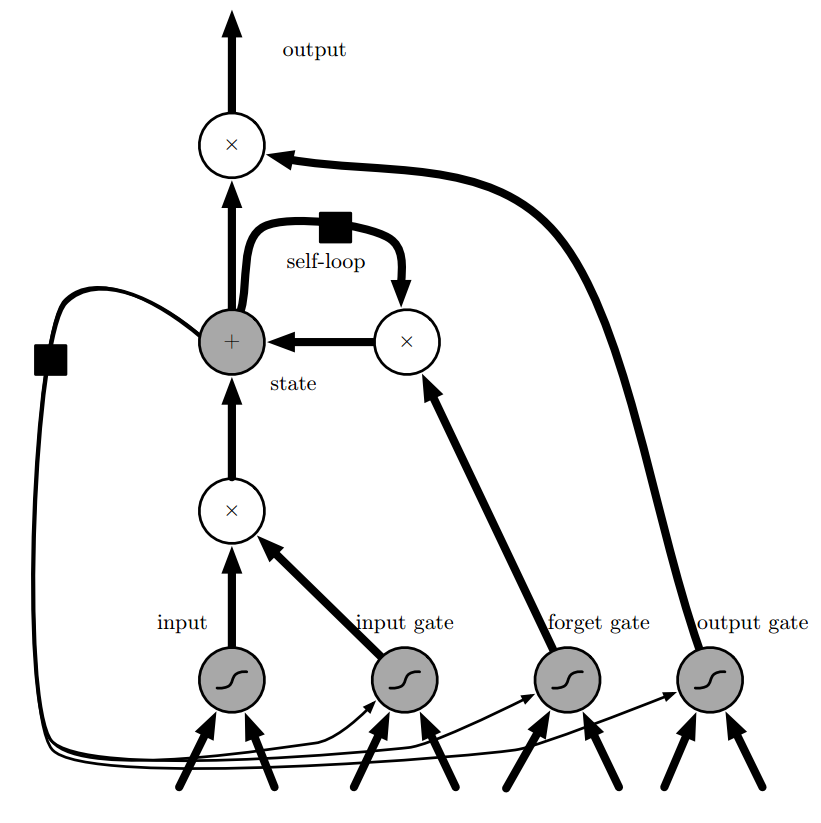
\includegraphics[scale=0.3]{figures/chapter_2/LSTM_cell.png}
	\caption{\glssymbol{LSTM}~\gls{recurrent_network}``细胞''的框图。
		细胞彼此循环连接,代替一般\gls{recurrent_network}中普通的\gls{hidden_unit}。
		这里使用常规的人工神经元计算输入特征。
		如果sigmoid输入门允许,它的值可以累加到状态。
		状态单元具有线性自循环,其权重由\gls{forget_gate}控制。
		细胞的输出可以被输出门关闭。
		所有\gls{gated}单元都具有sigmoid非线性,而输入单元可具有任意的压缩非线性。
		状态单元也可以用作\gls{gated}单元的额外输入。
		黑色方块表示单个\gls{time_step}的延迟。
	}\label{fig:chapter2_lstm_cell}
\end{figure}

\glssymbol{LSTM}~块如\figref{fig:chapter2_lstm_cell}所示。
在浅\gls{recurrent_network}的架构下,相应的\gls{forward_propagation}公式如下。
更深的架构也被成功应用\citep{Graves-et-al-ICASSP2013,Pascanu-et-al-ICLR2014}。
\glssymbol{LSTM}~\gls{recurrent_network}除了外部的~\glssymbol{RNN}~循环外,还具有内部的``\glssymbol{LSTM}~细胞''循环(自环),因此~\glssymbol{LSTM}~不是简单地向输入和循环单元的仿射变换之后施加一个逐元素的非线性。
与普通的\gls{recurrent_network}类似,每个单元有相同的输入和输出,但也有更多的参数和控制信息流动的\gls{gated}单元系统。

最重要的组成部分是状态单元$s_i^{(t)}$,与前一节讨论的\gls{leaky_unit}有类似的线性自环。
然而,此处自环的权重(或相关联的时间常数)由\firstgls{forget_gate}~$f_i^{(t)}$控制(时刻$t$和细胞$i$),由~\ENNAME{sigmoid}~单元将权重设置为0和1之间的值:

\begin{equation}
f_i^{(t)} = \sigma \Big( b_i^f + \sum_j U_{i,j}^f x_j^{(t)} + \sum_j W_{i,j}^f h_j^{(t-1)} \Big),
\end{equation}

其中$x^{(t)}$是当前输入向量,$h^{t}$是当前隐藏层向量,$h^{t}$包含所有~\glssymbol{LSTM}~细胞的输出。 
$b^f, U^f, W^f$分别是\gls{bias_aff}、输入权重和\gls{forget_gate}的循环权重。
因此~\glssymbol{LSTM}~细胞内部状态以如下方式更新,其中有一个条件的自环权重$f_i^{(t)}$:

\begin{align}
s_i^{(t)} = f_i^{(t)}  s_i^{(t-1)} +  g_i^{(t)}
\sigma \Big( b_i + \sum_j U_{i,j} x_j^{(t)} + \sum_j W_{i,j} h_j^{(t-1)} \Big),
\end{align}

其中$b, U, W$分别是~\glssymbol{LSTM}~细胞中的\gls{bias_aff}、输入权重和\gls{forget_gate}的循环权重。
\textbf{外部输入门}(external input gate)单元$g_i^{(t)}$以类似\gls{forget_gate}(使用\ENNAME{sigmoid}获得一个0和1之间的值)的方式更新,但有自身的参数:

\begin{align}
g_i^{(t)} = \sigma \Big( b_i^g + \sum_j U_{i,j}^g x_j^{(t)} + \sum_j W_{i,j}^g h_j^{(t-1)} \Big).
\end{align}

\glssymbol{LSTM}~细胞的输出$h_i^{(t)}$也可以由\textbf{输出门}(output gate)~$q_i^{(t)}$关闭(使用\ENNAME{sigmoid}单元作为\gls{gated}):

\begin{align}
h_i^{(t)} &= \text{tanh}\big( s_i^{(t)} \big) q_i^{(t)}, \\
q_i^{(t)} &= \sigma \Big( b_i^o + \sum_j U_{i,j}^o x_j^{(t)} + \sum_j W_{i,j}^o h_j^{(t-1)} \Big),
\end{align}

其中$b^o, U^o, W^o$分别是\gls{bias_aff}、输入权重和\gls{forget_gate}的循环权重。
在这些变体中,可以选择使用细胞状态$s_i^{(t)}$作为额外的输入(及其权重),输入到第$i$个单元的三个门,如\figref{fig:chapter2_lstm_cell}所示。
这将需要三个额外的参数。

\glssymbol{LSTM}~网络比简单的循环架构更易于学习\gls{long_term_dependency},先是用于测试\gls{long_term_dependency}学习能力的人工数据集\citep{Bengio-trnn94,Hochreiter+Schmidhuber-1997,chapter-gradient-flow-2001},然后是在具有挑战性的序列处理任务上获得最先进的表现\citep{Graves-book2012,Graves-arxiv2013,Sutskever-et-al-NIPS2014}。

\section{神经网络优化算法}
用于深度模型训练的优化算法与传统的优化算法在几个方面有所不同。 机器学习通常是间接作用的。
在大多数机器学习问题中,我们关注某些性能度量 P,其定义于测试集上并且可能是不可解的。
因此,我们只是间接地优化 P。我们希望通过降低代价函数$J(θ)$来提高 P。
这一点与纯优化不同,纯优化最小化目标 J 本身。训练深度模型的优化算法通常也会包括一些针对机器学习目标函数的特定结构进行的特化。

\subsection{\glsentrytext{SGD}优化算法}
\label{sec:stochastic_gradient_descent_chap8}
\gls{SGD}及其变种很可能是一般\gls{ML}中应用最多的优化算法,特别是在\gls{DL}中。
按照\gls{DGD}抽取$m$个\gls{minibatch}(独立同分布的)样本,通过计算它们梯度均值,
我们可以得到梯度的\gls{unbiased}估计。
展示了如何沿着这个梯度的估计下降。

\begin{algorithm}[ht]
	\caption{\gls{SGD}(\glssymbol{SGD})在第$k$个训练迭代的更新}
	\label{alg:sgd}
	\begin{algorithmic}
		\REQUIRE \gls{learning_rate} $\epsilon_k$
		\REQUIRE 初始参数$\theta$
		\WHILE{停止\gls{criterion}未满足}
		\STATE 从\gls{training_set}中采包含$m$个样本$\{ x^{(1)},\dots, x^{(m)}\}$ 的\gls{minibatch},其中$x^{(i)}$对应目标为$y^{(i)}$
		\STATE 计算梯度估计: $\hat{g} \leftarrow + 
		\frac{1}{m} \nabla_{\theta} \sum_i L(f(x^{(i)};\theta),y^{(i)})$
		\STATE 应用更新:$\theta \leftarrow theta - \epsilon \hat{g}$
		\ENDWHILE
	\end{algorithmic}
\end{algorithm}

\glssymbol{SGD}\,算法中的一个关键参数是\gls{learning_rate}。
之前,我们介绍的\,\glssymbol{SGD}\,使用固定的\gls{learning_rate}。
在实践中,有必要随着时间的推移逐渐降低\gls{learning_rate},
因此我们将第$k$步迭代的\gls{learning_rate}记作$\epsilon_k$。

这是因为\,\glssymbol{SGD}\,中梯度估计引入的噪声源($m$个训练样本的随机采样)并不会在\gls{minimum}处消失。
相比之下,当我们使用\gls{batch}\gls{GD}到达\gls{minimum}时,整个\gls{cost_function}的真实梯度会变得很小,
之后为$\mathbf{0}$,因此\gls{batch}\gls{GD}可以使用固定的\gls{learning_rate}。
保证\,\glssymbol{SGD}\,收敛的一个充分条件是
\begin{equation}
\label{eq:8.12}
\sum_{k=1}^\infty \epsilon_k = \infty,
\end{equation}
且
\begin{equation}
\label{eq:8.13}
\sum_{k=1}^\infty \epsilon_k^2 < \infty.
\end{equation}

实践中,一般会线性衰减\gls{learning_rate}直到第$\tau$次迭代:
\begin{equation}
\label{eq:8.14}
\epsilon_k = (1-\alpha) \epsilon_0 + \alpha \epsilon_\tau
\end{equation}
其中$\alpha = \frac{k}{\tau}$。
在$\tau$步迭代之后,一般使$\epsilon$保持常数。

\subsection{RMSProp优化算法}
\label{sec:rmsprop}
\textbf{RMSProp}算法\citep{Hinton-ipam2012}修改AdaGrad以在\gls{nonconvex}设定下效果更好,
改变梯度积累为指数加权的移动平均。
\gls{adagrad}\,旨在应用于凸问题时快速收敛。
当应用于\gls{nonconvex}函数训练\gls{NN}时,学习轨迹可能穿过了很多不同的结构,最终到达一个局部是凸碗的区域。
AdaGrad根据平方梯度的整个历史收缩\gls{learning_rate},可能使得\gls{learning_rate}在达到这样的凸结构前就变得太小了。
RMSProp使用指数衰减平均以丢弃遥远过去的历史,使其能够在找到凸碗状结构后快速收敛,
它就像一个初始化于该碗状结构的AdaGrad算法实例。

RMSProp的标准形式如\algref{alg:rms_prop}所示,结合Nesterov动量的形式如\algref{alg:rms_nesterov}所示。
相比于AdaGrad,使用移动平均引入了一个新的\gls{hyperparameter}$\rho$,用来控制移动平均的长度范围。

经验上,RMSProp已被证明是一种有效且实用的\gls{DNN}优化算法。
目前它是\gls{DL}从业者经常采用的优化方法之一。


\begin{algorithm}[ht]
	\caption{RMSProp算法}
	\label{alg:rms_prop}
	\begin{algorithmic}
		\REQUIRE 全局\gls{learning_rate} $\epsilon$,衰减速率$\rho$
		\REQUIRE  初始参数$\theta$
		\REQUIRE 小常数$\delta$,通常设为$10^{-6}$(用于被小数除时的数值稳定)
		\STATE 初始化累积变量 $r = 0$
		\WHILE{没有达到停止\gls{criterion}}
		\STATE 从\gls{training_set}中采包含$m$个样本$\{ x^{(1)},\dots, x^{(m)}\}$ 的\gls{minibatch},对应目标为$y^{(i)}$。
		\STATE 计算梯度:$g \leftarrow  
		\frac{1}{m} \nabla_{\theta} \sum_i L(f(x^{(i)};\theta),y^{(i)})$ 
		\STATE 累积平方梯度:$r \leftarrow \rho
		r + (1-\rho) g \odot g$
		\STATE 计算参数更新:$\Delta \theta =
		-\frac{\epsilon}{\sqrt{\delta + r}} \odot g$  \ \  ($\frac{1}{\sqrt{\delta + r}}$ 逐元素应用)
		\STATE 应用更新:$\theta \leftarrow \theta + \Delta \theta$
		\ENDWHILE
	\end{algorithmic}
\end{algorithm}

\subsection{Adam}
\label{sec:adam}
\textbf{Adam}~\citep{kingma2014adam}是另一种\gls{learning_rate}自适应的优化算法,如\algref{alg:adam}所示。
``Adam''这个名字派生自短语``adaptive moments''。
早期算法背景下,它也许最好被看作结合RMSProp和具有一些重要区别的\gls{momentum}的变种。
首先,在Adam中,\gls{momentum}直接并入了梯度一阶矩(指数加权)的估计。
将\gls{momentum}加入RMSProp最直观的方法是将\gls{momentum}应用于缩放后的梯度。
结合缩放的\gls{momentum}使用没有明确的理论动机。
其次,Adam包括偏置修正,修正从原点初始化的一阶矩(\gls{momentum}项)和(非中心的)二阶矩的估计(\algref{alg:adam})。
RMSProp也采用了(非中心的)二阶矩估计,然而缺失了修正因子。
因此,不像Adam,RMSProp二阶矩估计可能在训练初期有很高的偏置。
Adam通常被认为对\gls{hyperparameter}的选择相当鲁棒,尽管\gls{learning_rate}有时需要从建议的默认修改。

\begin{algorithm}[ht]
	\caption{Adam算法}
	\label{alg:adam}
	\begin{algorithmic}
		\REQUIRE 步长 $\epsilon$ (建议默认为: $0.001$)
		\REQUIRE 矩估计的指数衰减速率, $\rho_1$ 和 $\rho_2$ 在区间 $[0, 1)$内。
		(建议默认为:分别为$0.9$ 和 $0.999$)
		\REQUIRE 用于数值稳定的小常数 $\delta$  (建议默认为: $10^{-8}$)
		\REQUIRE 初始参数 $\theta$
		\STATE 初始化一阶和二阶矩变量 $s = 0 $, $r = 0$
		\STATE 初始化\gls{time_step} $t=0$ 
		\WHILE{没有达到停止\gls{criterion}}
		\STATE 从\gls{training_set}中采包含$m$个样本$\{ x^{(1)},\dots, x^{(m)}\}$ 的\gls{minibatch},对应目标为$y^{(i)}$。
		\STATE 计算梯度:$g \leftarrow \frac{1}{m} \nabla_{\theta} \sum_i L(f(x^{(i)};\theta),y^{(i)})$ 
		\STATE $t \leftarrow t + 1$
		\STATE 更新有偏一阶矩估计: $s \leftarrow \rho_1 s + (1-\rho_1) g$
		\STATE 更新有偏二阶矩估计:$r \leftarrow \rho_2 r + (1-\rho_2)  g \odot g$
		\STATE 修正一阶矩的\gls{bias_sta}:$\hat{s} \leftarrow \frac{s}{1-\rho_1^t}$
		\STATE 修正二阶矩的\gls{bias_sta}:$\hat{r} \leftarrow \frac{r}{1-\rho_2^t}$
		\STATE 计算更新:$\Delta \theta = - \epsilon \frac{\hat{s}}{\sqrt{\hat{r}} + \delta}$ \ \  (逐元素应用操作)
		\STATE 应用更新:$\theta \leftarrow \theta + \Delta \theta$
		\ENDWHILE
	\end{algorithmic}
\end{algorithm}

\subsection{选择正确的优化算法}
\label{sec:choosing_the_right_optimization_algorithms}
在本节中,我们讨论了一系列算法,通过自适应每个模型参数的\gls{learning_rate}以解决优化\gls{deep_model}中的难题。
此时,一个自然的问题是:该选择哪种算法呢?

遗憾的是,目前在这一点上没有达成共识。
\cite{Schaul2014_unittests}展示了许多优化算法在大量学习任务上极具价值的比较。
虽然结果表明,具有自适应\gls{learning_rate}(以RMSProp和AdaDelta为代表)的算法族表现得相当鲁棒,不分伯仲,但没有哪个算法能脱颖而出。

目前,最流行并且使用很高的优化算法包括SGD、具\gls{momentum}的SGD、RMSProp、具\gls{momentum}的RMSProp、AdaDelta和Adam。
此时,选择哪一个算法似乎主要取决于使用者对算法的熟悉程度(以便调节\gls{hyperparameter})。

\section{本章小结}